\chapter{Stand der Forschung und technische Grundlagen}
\label{ch:stand_der_forschung}
Dieses Kapitel dient dem Überblick über die für diese Arbeit relevanten Forschungsgebiete und ihre Methoden. Außerdem werden technische Grundlagen erläutert. Zunächst erfolgt eine Einführung in das Forschungsfeld der Kontinuumsrobotik. Insbesondere richtet sich der Fokus auf etablierte Modelle zur kinematischen Beschreibung kontinuierlicher Manipulatoren. Eine Formulierung der Vorwärtskinematik für den in dieser Arbeit modellierten kontinuierlichen Manipulator findet statt. Die Vorwärtskinematik ist der Ausgangspunkt für die Datengenerierung zur Ermittlung der Inverskinematik mittels maschinellem Lernen im Hauptteil dieser Arbeit. Bereits bestehende Möglichkeiten, die inverse Kinematik zu beschreiben, werden aufgeführt.
%In diesem Zusammenhang findet ein Vergleich unterschiedlicher Darstellungen von Orientierungen eines Körpers im kartesischen Raum statt. 
Anschließend werden relevante Methoden und Konzepte des \textit{Reinforcement Learning} beschrieben. Insbesondere wird die Approximation von Funktionen mittels künstlicher neuronaler Netzwerke beschrieben. Abschließend erfolgt eine Abgrenzung der bestehenden, inversen Kinematikmodelle zu dem in dieser Arbeit herausgearbeiteten Vorgehen. 

%Wesentliche Bestandteile des RL bilden der episodische \textit{Markov Decision Process} (MDP) sowie die allgemeine Zielsetzung den zukünftig, erwarteten \textit{reward} zu maximieren.

%Zuletzt wird der in dieser Arbeit verwendete Ansatz zur Lösung der inversen Kinematik eines aus zwei Segmenten bestehenden seilzugaktuierten Kontinuumsroboters vorgestellt und mit bereits existierenden Lösungen verglichen.

\section{Kontinuumsrobotik}
\label{sec:kontinuumsrobotik}

Der Ursprung der Kontinuumsrobotik lässt sich auf die Sechzigerjahre des 20. Jahrhunderts zurückführen. Im Jahr 1968 ließen sich Anderson und Horn den \textit{Tensor arm manipulator}\footnote{https://patents.google.com/patent/US3497083 (aufgerufen am 25.07.2018)}, der mithilfe von insgesamt 40 Seilzügen und zehn miteinander verbundenen Platten aktuiert wird, patentieren. Der \textit{Tensor arm manipulator} gilt als einer der ersten Kontinuumsroboter~\cite{Wal13}. Oftmals dienen Vorbilder aus dem Tierreich als Inspiration für die Gestaltung kontinuierlicher Manipulatoren. Elefantenrüssel, Tentakel von Kraken und Schlangen bilden prominente Beispiele, welche gemeinsam mit ihren nachgebildeten Robotern in Bild~\ref{fig:tiere_roboter} illustriert sind. Bei den Nachbildungen geht es nicht vorrangig darum, das Vorbild aus der Natur möglichst genau zu kopieren. Stattdessen versucht man, die herausragenden Eigenschaften von Tieren in der Domäne der Robotik umzusetzen und sich zunutze zu machen. Die bedeutendste Eigenschaft kontinuierlicher Manipulatoren ist ihre Flexibilität und Nachgiebigkeit, die es ihnen ermöglicht, sich kontinuierlich zu krümmen. Dieses Merkmal ist ein wesentlicher Bestandteil verschiedener Definitionen von Kontinuumsrobotern. Im Jahr 1999 definieren Robinson und Davies~\cite{RD99}:

\begin{figure}[t!]
% alle bilder sind ausgeschnitten mit 640 x 427 pixels
\centering
\subcaptionbox{Elefantenrüssel\protect\footnotemark}%
[.32\linewidth]{\includegraphics[width=.32\linewidth]{bilder/standdertechnik/elephant_trunk_crop.jpg}}
\subcaptionbox{Oktopus\protect\footnotemark}%
[.32\linewidth]{\includegraphics[width=.32\linewidth]{bilder/standdertechnik/octopus.jpg}}
\subcaptionbox{Schlange\protect\footnotemark}
[.32\linewidth]{\includegraphics[width=.32\linewidth]{bilder/standdertechnik/snake.jpg}}
\medskip
\subcaptionbox{\textit{\textit{Elephant trunk manipulator}}\cite{WH99}}%
[.32\linewidth]{\includegraphics[width=.32\linewidth]{bilder/standdertechnik/elephant_trunk_robot2_crop.png}}
\subcaptionbox{OctArm \cite{COW08}\label{sf:octarm_grap}}%
[.32\linewidth]{\includegraphics[width=.32\linewidth]{bilder/standdertechnik/octarm2_crop.png}}
\subcaptionbox{ACM-R3 \cite{HY09}}
[.32\linewidth]{\includegraphics[width=.32\linewidth]{bilder/standdertechnik/acm_r3_crop.png}}
\caption[Vorbilder für Kontinuumsroboter aus dem Tierreich und an sie angelehnte Nachbildungen]{Vorbilder für Kontinuumsroboter aus dem Tierreich und an sie angelehnte Nachbildungen}
\label{fig:tiere_roboter}
\end{figure}

\begin{quotation}
\textit{Continuum robots do not contain rigid links and identifiable rotational joints. Instead the structures bend continuously along their length via elastic deformation and produce motion through the generation of smooth curves, similar to tentacles or tongues of the animal kingdom.}
\end{quotation}

Auch die Definition von Walker im Jahr 2013 greift diesen Punkt auf und grenzt kontinuierliche Manipulatoren zusätzlich von seriellen Robotern ab~\cite{Wal13}:

\begin{quotation}
\textit{These robots, termed continuum robots, can be viewed as being ``invertebrate`` robots, as compared with ``vertebrate`` design of conventional rigid-link robots. Continuum robots can bend (and often extend/contract and sometimes twist) at any point along their structure.}
\end{quotation}

%%%%%%%%%%%%%%%%%%%%%%%%%%%%%%%%%%%%%%%%%%%%%%%%%%%%%%%%%%%%%%%%%%%%
\footnotetext[2]{https://commons.wikimedia.org/wiki/File:Elephant\_trunk\_(1).jpg (aufgerufen am 26.07.2018)}
\footnotetext[3]{https://commons.wikimedia.org/wiki/File:Pinnoctopus\_cordiformis.jpg (aufgerufen am 26.07.2018)}
\footnotetext[4]{https://commons.wikimedia.org/wiki/File:Chrysopelea\_taprobanica.jpg (aufgerufen am 26.07.2018)}
%%%%%%%%%%%%%%%%%%%%%%%%%%%%%%%%%%%%%%%%%%%%%%%%%%%%%%%%%%%%%%%%%%%%%

Eine aktuellere Definition von Burgner und Rucker aus dem Jahr 2015 verallgemeinert den Begriff des Kontinuumsroboters wie folgt~\cite{BRC15}:

\begin{quotation}
\textit{A continuum robot is an actuatable structure whose constitutive material forms curves with continuous tangent vectors.}
\end{quotation}

Die oben aufgeführten Definitionen grenzen direkt und indirekt Kontinuumsroboter von den in der Industrie etablierten rigiden, seriellen Robotern ab. Anstelle von steifen, über Gelenke miteinander verbundenen Gliedern besitzen Kontinuumsroboter oft ein sich kontinuierlich biegsames Rückgrat. Eine daraus abgeleitete und erwünschte Eigenschaft kontinuierlicher Manipulatoren lautet, in schwer zugänglichen Umgebungen navigieren und manövrieren zu können. Die inhärente Nachgiebigkeit unterstützt die Fähigkeit, sich in gewundenen Hohlräumen der äußeren Struktur anzupassen. Kontinuumsroboter unterscheiden sich zusätzlich von seriellen Robotern in der Art und Weise, wie sie ihre Umwelt manipulieren können. Während serielle Roboter mittels speziell angefertigter Endeffektoren Gegenstände greifen und bewegen, sollen kontinuierliche Roboter ähnlich wie Elefantenrüssel oder Tentakel zusätzlich in der Lage sein, Gegenstände mit ihrer gesamten Struktur zu umschließen~\cite{Moc01}, siehe Bild~\ref{fig:tiere_roboter}\,(e).

Walker unterteilt in~\cite{Wal13} kontinuierliche Manipulatoren in drei durch ihr Design und ihre Aktuierung bestimmte Gruppen. Die erste Gruppe bilden \textit{seilzugaktuierte Kontinuumsroboter}, welche durch Verkürzen und Verlängern von Seilzügen, die entlang des kontinuierlichen Manipulators angebracht sind, die Form des Roboters bestimmen. 

Zur zweiten Gruppe gehören \textit{tubuläre Kontinuumsroboter}. Bei dem tubulären Kontinuumsroboter mehrere konzentrisch ineinander verbaute Röhrchen bewegt und rotiert, um Translationen und Torsionen des Endeffektors zu erzeugen. Mittels einer zusätzlichen Vorbiegung der Röhrchen ist es möglich, eine kontinuierliche Krümmung zu erzeugen. 
Die ersten beiden Gruppen werden extrinsische Manipulatoren genannt, da die Aktorik außerhalb von dem eigentlichen Manipulator angebracht ist. Eine Folge der extrinsischen Aktuierung ist die Realisierung kompakter und filigraner Designs des eigentlichen Manipulators. 

Die dritte Gruppe von Robotern gehört zu den intrinsischen Manipulatoren und Walker nennt diese \textit{lokal aktuierte Rückgratdesigns}. Hier sind die Aktoren Teil der eigentlichen Rückgratstruktur und somit direkt an der Formgebung beteiligt. Sogenannte pneumatisch bewegte \textit{McKibben-Muskeln} können hier als Aktoren dienen. Jeweils ein Beispiel der oben angegebenen Gruppen ist in Bild~\ref{fig:drei_kontinuumsroboter} zu sehen. \newline

Im Rahmen dieser Arbeit wird ein seilzugaktuierter Kontinuumsroboter bestehend aus zwei Segmenten kinematisch modelliert, da dieser den kontinuierlichen kinematischen Ketten im Forschungsprojekt \textit{Parallel-kontinuierliche Manipulatoren} des \textit{Lehrstuhls für Kontinuumsrobotik} und des \textit{Instituts für mechatronische Systeme} ähnelt. An jedem Segment enden jeweils drei Seilzüge, wodurch der Roboter insgesamt sechs Freiheitsgrade aufweist. Grundsätzliche Eigenschaften der Kinematik sind Gegenstand des nächsten Abschnitts.

\begin{figure}[t!]
% all pictures are resized to 640 x 480 pixels
\centering
\subcaptionbox{Seilzugaktuierter \\Manipulator~\cite{NB16}}[.32\linewidth]
{\includegraphics[width=.32\linewidth]{bilder/standdertechnik/tendon_driven_continuum_robot_resized.png}}
\label{fig:seilzugaktuiert}
\subcaptionbox{Tubulärer \\Manipulator~\cite{BRG+14}}[.32\linewidth]
{\includegraphics[width=.32\linewidth]{bilder/standdertechnik/tubular_resize.png}}
\label{fig:tubulaer}
\subcaptionbox{Pneumatisch aktuierter \\ Manipulator~\cite{BKW13}}[.32\linewidth]
{\includegraphics[width=.32\linewidth]{bilder/standdertechnik/mckibben_resize.png}}
\caption[Prominente Beispiele der Kontinuumsrobotik]{Prominente Beispiele der Kontinuumsrobotik}
\label{fig:drei_kontinuumsroboter}
\end{figure}



\pagebreak
\section{Kinematik kontinuierlicher Manipulatoren}
\label{sec:kinematik_allgemein}

Nachfolgend werden kinematische Beziehungen im Hinblick auf kontinuierliche Manipulatoren erläutert. Im Allgemeinen bezeichnet die Vorwärts- oder direkte Kinematik 
%
\begin{equation}
\label{eq:vorwaertskinematik}
\bm{x}_\mathrm{E} = \bm{f}(\bm{q}) 
\end{equation}
%
den geometrischen Zusammenhang zwischen den Gelenkwinkeln des Roboters $\bm{q}$ und der daraus resultierenden Position und Orientierung des Endeffektors $\bm{x}_\mathrm{E}$. Mit~\eqref{eq:vorwaertskinematik} wird der Gelenkraum des Roboters auf den kartesischen Arbeitsraum abgebildet. Bei $m$ Gelenkwinkeln ergibt sich:
$\bm{q} = \left[q_1, q_2, ..., q_m \right]^\transpose$. 
Wird im Folgenden von der Lage des Endeffektors gesprochen, werden sowohl dessen Position als auch Orientierung beachtet. 
Zur Beschreibung der alleinigen Position~$\bm{x}_{\mathrm{E,p}} = \left[ x_\mathrm{E}, y_\mathrm{E}, z_\mathrm{E} \right]^\transpose$ werden kartesische Raumkoordinaten verwendet.
Orientierungen bzw. Drehlagen des Endeffektors können auf unterschiedliche Art und Weise beschrieben werden. Im Allgemeinen wird die Variable der Orientierung mit dem entsprechenden Subskript~$\bm{x}_{\mathrm{E,o}}$ versehen .
%Mithilfe von drei \mbox{Winkeln $\varphi_\mathrm{E}, \psi_\mathrm{E}, \theta_\mathrm{E}$} zur Darstellung der Orientierung und den kartesischen Koordinaten $x_\mathrm{E}, y_\mathrm{E}, z_\mathrm{E}$ der Position lässt sich die Lage des Endeffektors exemplarisch folgendermaßen beschreiben: \mbox{$\bm{x}_\mathrm{E} = \left[x_\mathrm{E}, y_\mathrm{E}, z_\mathrm{E}, \varphi_\mathrm{E}, \psi_\mathrm{E}, \theta_\mathrm{E} \right]^\transpose $}. Zur Beschreibung der alleinigen Position bzw. Orientierung des Endeffektors wird die Variable $\bm{x}_{\mathrm{E,p}}$ respektive $\bm{x}_{\mathrm{E,o}}$ verwendet.  
Der Begriff der Kinematik lässt sich auch auf die zeitlichen Ableitungen von~\eqref{eq:vorwaertskinematik} ausweiten. Die direkte Kinematik für Gelenkwinkelgeschwindigkeiten und -beschleunigungen beschreibt den vereinfachten Zusammenhang \mbox{$\bm{\dot{q}} \Leftrightarrow \bm{\dot{x}}_\mathrm{E}$} bzw. \mbox{$\bm{\ddot{q}} \Leftrightarrow \bm{\ddot{x}}_\mathrm{E}$}. Variablen mit hochgestellten Punkten stellen die zeitlichen Ableitungen der jeweiligen Größe dar. 
Im Rahmen dieser Arbeit wird für die Ermittlung der Inverskinematik der zeitunabhängige Zusammenhang untersucht. 

Für die Vorwärtskinematik unterschiedlicher Kontinuumsroboter existieren etablierte Modelle, die in~\cite{WIJ10} zusammengefasst sind.
Ein Großteil der in der Literatur dokumentierten Kinematiken nehmen an, dass der betrachtete kontinuierliche Manipulator eine stückweise konstante Krümmung aufweist. 
Das bedeutet, dass sich die Form des Roboters mittels mehrerer, miteinander verknüpfter Kreissegmente im Raum beschreiben lässt. Diese Annahme stellt zwar nur eine Approximation der tatsächlichen Roboterstruktur dar, wird jedoch in der Forschung vielfach appliziert~\cite{HW03}, \cite{STF04}, \cite{JW06a}, \cite{RJWRC09}, \cite{DLIB10}. 
Die Tangentenvektoren am Kopplungspunkt zweier Kreissegmente sind jeweils identisch. Dieser Punkt wird auch in der oben aufgeführten Definition von Burgner und Rucker zu Kontinuumsrobotern aufgenommen.
Des Weiteren ermöglicht die Annahme der stückweise konstanten Krümmung eine Unterteilung der Vorwärts- und Inverskinematik in einen roboterspezifischen und roboterunabhängigen Teil~\cite{WIJ10}. 

Der roboterspezifische Zusammenhang beschreibt die Verknüpfung zwischen Gelenkwinkeln des Roboters und daraus abgeleiteten Bogenparametern, die einen Kreisabschnitt beschreiben. Die roboterunabhängige Funktion ermittelt aus den Bogenparametern die Position und Orientierung entlang des Kreisbogens.
Die unterschiedlichen kinematischen Räume sowie ihre Beziehung zueinander sind in Bild~\ref{fig:kinematikraeume} veranschaulicht. In den folgenden Abschnitten werden die einzelnen kinematischen Komponenten zunächst für ein Segment eines kontinuierlichen Manipulators erläutert. Im Anschluss wird gezeigt, wie mehrere Transformationen verknüpft werden.  

\begin{figure}[htb!] % 
\centering
\begin{tikzpicture}[auto, node distance=4cm]
% Erzeuge Boxen mit innerem Text
\node[simplebox, minimum size=1.5cm, name=arcparams, label={[align=center]:Bogen-\\ parameter}, label={[align=center]below:Konfigurations-\\ raum}] {\textblack{$\kappa, \phi, l$}};
\node[simplebox, minimum size=1.5cm, node distance=5cm, left of=arcparams, name=q, label={[align=center]:Seil-\\ längen}, label={[align=center]below:Gelenk-\\ raum}] {\textblack{$\bm{q}$}};
\node[simplebox, minimum size=1.5cm, node distance=5cm, right of=arcparams, name=x, label={[align=center]:Position,\\ Orientierung}, label={[align=center]below:Arbeits-\\ raum}] {\textblack{$\bm{x}_\mathrm{E}$}};
% berechne Punkte für verschobene Linien zwischen Boxen
\path (arcparams.east) -- (arcparams.north east) coordinate[pos=0.5] (arcparamsrighttop);
\path (arcparams.east) -- (arcparams.south east) coordinate[pos=0.5] (arcparamsrightbottom);
\path (arcparams.west) -- (arcparams.north west) coordinate[pos=0.5] (arcparamslefttop);
\path (arcparams.west) -- (arcparams.south west) coordinate[pos=0.5] (arcparamsleftbottom);
\path (q.east) -- (q.north east) coordinate[pos=0.5] (q1);
\path (q.east) -- (q.south east) coordinate[pos=0.5] (q2);
\path (x.west) -- (x.north west) coordinate[pos=0.5] (x1);
\path (x.west) -- (x.south west) coordinate[pos=0.5] (x2);
% zeichne Pfeile zwischen den Boxen
\draw[simplearrow] (q1) to node [align=center] {\textblack{$\bm{f}_{\text{s}}(\bm{q})$}}      (arcparamslefttop);
\draw[simplearrow] (arcparamsleftbottom) to node [align=center] {\textblack{$\bm{f}^{-1}_{\text{s}}(\kappa, \phi, l)$}} (q2);
\draw[simplearrow] (x2) to node [align=center] {\textblack{$\bm{f}^{-1}_{\text{u}}(\bm{x}_\mathrm{E})$}}      (arcparamsrightbottom);
\draw[simplearrow] (arcparamsrighttop) to node [align=center] {\textblack{$\bm{f}_{\text{u}}(\kappa, \phi, l)$}} (x1);
\end{tikzpicture}
\caption[Grafische Darstellung der kinematischen Räume eines Kontinuumsroboters mit stückweise konstanter Krümmung]{Grafische Darstellung der kinematischen Räume eines Kontinuumsroboters mit stückweise konstanter Krümmung in Anlehnung an \cite{WIJ10}}
\label{fig:kinematikraeume}
\end{figure}


\subsection{Roboterunabhängige Vorwärtskinematik}
\label{subsec:unabhaengige_vorwaertskinematik}

Zunächst soll in diesem Abschnitt die roboterunabhängige Kinematik für ein einzelnes kontinuierliches Segment untersucht werden. Das Ziel ist es, die Position und Orientierung eines Kreisabschnitts mithilfe von Bogenparametern zu beschreiben. Der ermittelte Kreisabschnitt approximiert die Form des Kontinuumsroboters. \newline

Die roboterunabhängige Vorwärtskinematik
\begin{align}
\bm{x}_\mathrm{E} = \bm{f}_{\text{u}}(\kappa, \phi, \ell) 
\label{eq:funabhaengig}
\end{align}

beschreibt formal den Zusammenhang zwischen den Bogenparametern $\kappa, \phi, \ell$ und der Lage des Endeffektors $\bm{x}_{\mathrm{E}}.$ 
Es ist~\mbox{$\kappa = 1/r$} die Krümmung eines Kreissegments, wobei $r$ den Radius des Kreises beschreibt. Der Winkel $\phi$ rotiert den Kreisbogen aus der \mbox{$x$-$z$-Ebene}. Die Bogenlänge des Kreissegments lautet $\ell$. Um sämtliche Punkte auf dem Kreisbogen beschreiben zu können, wird die variable Bogenlänge \mbox{$c \in [0~\ell]$} eingeführt. In~\cite{WIJ10} sind insgesamt 5 verschiedene Vorgehensweisen für die Ermittlung der roboterunabhängigen Kinematik aufgeführt. Jedes dieser Verfahren lässt sich jedoch auf dasselbe Ergebnis überführen, nämlich eine homogene Transformationsmatrix, die mit der variablen Bogenlänge $c$ sämtliche Lagen auf dem Kreisbogen beschreiben kann. In dieser Arbeit wird die geometrische Herleitung der direkten roboterunabhängigen Kinematik aufgrund ihrer Einfachheit näher beleuchtet. 

Ausgangspunkt der geometrischen Betrachtung ist ein Kreisbogen, welcher in der \mbox{$x$-$z$-Ebene} liegt. Es befindet sich ein Ende des Abschnitts im Ursprung. Dieser Zustand ist in Bild~\ref{fig:bogenparameter}\,(a) dargestellt. Der Kreisbogen ist um den \mbox{Winkel $\theta \in [0~2\pi]$} aus dem Ursprung rotiert. 
%Es \mbox{gilt $\kappa = \theta c$}. 
Die Koordinaten des Punktes lauten: \mbox{$\bm{p} = [r(1-\cos\theta),0,r\sin\theta]^\transpose$}.
Anschließend wird der Punkt $\bm{p}$ aus der \mbox{$x$-$z$-Ebene} um den \mbox{Winkel~$\phi\in[0~2\pi]$} und die \mbox{$z$-Achse} rotiert, sodass man die Lage des Endeffektors $\bm{x}_{\mathrm{E}}$ erhält, wie in Bild~\ref{fig:bogenparameter}\,(b) zu sehen ist. 

\begin{figure}[hbt!]
\centering
\subcaptionbox{Bogengeometrie in der $x$-$z$-Ebene}[.48\linewidth]
{\input{bilder/standdertechnik/arc_geometry.pdf_tex}}
\label{fig:bogengeometrie}
\subcaptionbox[Bogenparameter eines Segments des Kontinuumsroboters]{Bogenparameter eines Segments des Kontinuumsroboters mit Darstellung der Rotationsebene}
{\input{bilder/standdertechnik/configuration_space02.pdf_tex}}
\caption[Geometrische Darstellung eines Kreissegments im kartesischen Raum]{Geometrische Darstellung eines Kreissegments im kartesischen Raum}
\label{fig:bogenparameter}
\end{figure}

Die aufgeführte Darstellung eines Kreisbogens lässt sich über die Verknüpfung von zwei Rotationen und einer Translation mathematisch zu einer homogenen Transformation zusammenfassen:
\begin{align}
\bm{T} = 
\begin{bmatrix}
\bm{R}_z(\phi) & \bm{0} \\
\bm{0} & 1
\end{bmatrix}
\begin{bmatrix}
\bm{R}_y(\theta) & \bm{p} \\
\bm{0} & 1
\end{bmatrix}.
\label{eq:T}
\end{align}

Die Rotationsmatrizen $\bm{R}_z(\phi)$ und $\bm{R}_y(\theta)$ beschreiben eine Elementardrehung der speziell orthogonalen Gruppe~$\mathrm{SO}(3)$ im dreidimensionalen Raum. Die Rotationsachse steht jeweils im Subskript und der Rotationswinkel im Argument der Rotationsmatrix. Mittels einer Erweiterung der Rotationsmatrix um eine Translation wird die affine, homogene Transformation gebildet, welche zu der euklidischen Gruppe~$\mathrm{SE}(3)$ gehört. Mit~\eqref{eq:T} und $\theta=\kappa c$ lässt sich die roboterunabhängige Transformationsmatrix aufstellen:
\begin{align}
%\bm{f}_\mathrm{u}(\kappa,\phi,c) =
\bm{T}_\mathrm{F} = 
\begin{bmatrix}
\cos\phi \cos\kappa c & -\sin\phi & \cos\phi \sin\kappa c & \frac{cos\phi (1-\cos\kappa c)}{\kappa} \\
\sin\phi \cos\kappa c & \cos\phi & \sin\phi \sin\kappa c & \frac{\sin\phi( (1-\cos\kappa c)}{\kappa} \\
-\sin\kappa c &  0 & \cos\kappa c & \frac{\sin\kappa c}{\kappa} \\
%%%%%%%%%%%%%%%%%%%%%%%%%%%%%%%%%% andere schreibweise der matrizen
%\cos\phi \cos\kappa c & -\sin\phi & \cos\phi \sin\kappa c & \cos\phi (1-\cos\kappa c)/\kappa \\
%\sin\phi \cos\kappa c &  \cos\phi & \sin\phi \sin\kappa c & \sin\phi (1-\cos\kappa c)/\kappa \\
%-\sin\kappa c &  0 & \cos\kappa c & \sin\kappa c / \kappa \\
0 & 0 & 0 & 1
\end{bmatrix}.
\label{eq:T_frenet}
\end{align}

Die \mbox{$x$-Achse} des mit~\eqref{eq:T_frenet} transformierten Koordinatensystems zeigt auf den Mittelpunkt des Kreisbogens. Damit wird das Koordinatensystem des Endeffektors im sogenannten \textit{Frenet-Serret}-Koordinatensystem, durch das Subskript $\mathrm{F}$ verdeutlicht, dargestellt. Dies impliziert, dass der kontinuierliche Manipulator einer Torsion ausgesetzt ist. Im Rahmen dieser Arbeit wird jedoch unterstellt, dass sich der seilzugaktuierte Roboter torsionsfrei krümmt. Durch eine nachträgliche Rechtsmultiplikation von~\eqref{eq:T_frenet} \mbox{mit $\bm{R}_z(-\phi)$} ohne Translation kann das Endeffektorkoordinatensystem torsionsfrei beschrieben werden~\cite{WIJ10}. Die neue Transformationsmatrix im \textit{Bishop}-Koordinatensystem mit Subskript $\mathrm{B}$ lautet:
\begin{align}
%&\bm{f}_{\mathrm{u}} (\kappa, \phi, c) = 
\bm{T}_\mathrm{B} &=  \bm{T}_{\mathrm{F}}
\begin{bmatrix}
\bm{R}_z\left( -\phi \right) & \bm{0}\\
\bm{0} & 1 
\end{bmatrix} \nonumber \\
&=\begin{bmatrix}
\cos^2\phi(cos\kappa c - 1)+1 & \sin\phi\cos\phi (\cos\kappa c -1) & \cos\phi \sin\kappa c & \frac{\cos\phi(1-\cos\kappa c)}{\kappa} \\
\sin\phi \cos\phi (\cos\kappa c-1) & \cos^2\phi(1-\cos\kappa c)+\cos\kappa c & \sin\phi \sin\kappa c & \frac{\sin\phi(1 \shortminus \cos\kappa c)}{\kappa} \\
-\cos\phi \sin\kappa c & -\sin\phi \sin\kappa c & \cos\kappa c & \frac{\sin\kappa c}{\kappa} \\
%%%%%%%%%%%%%%%%%%%%%%%%%%%%%%%%%% andere schreibweise der matrizen
%\cos^2\phi(cos\kappa c \shortminus 1)+1 & \sin\phi\cos\phi (\cos\kappa c \shortminus 1) & \cos\phi \sin\kappa c & cos\phi (1 \shortminus \cos\kappa c)/\kappa \\
%\sin\phi \cos\phi (\cos\kappa c \shortminus 1) & \cos^2\phi(1 \shortminus \cos\kappa c)+\cos\kappa c & \sin\phi \sin\kappa c & \sin\phi (1 \shortminus \cos\kappa c)/\kappa \\
%\shortminus \cos\phi \sin\kappa c & \shortminus \sin\phi \sin\kappa c & \cos\kappa c & \sin\kappa c / \kappa \\
0 & 0 & 0 & 1 
\end{bmatrix}.
\label{eq:T_bishop}
\end{align}

Mit~\eqref{eq:T_bishop} lässt sich nun ein beliebiger erweiterter Ortsvektor durch Linksmultiplikation torsionsfrei transformieren. 
Die Drehlage des Endeffektors kann mithilfe der Rotationsmatrix unterschiedlich dargestellt werden. Aus diesem Grund wird auf eine explizite Beschreibung der vektorwertigen Funktion~\eqref{eq:funabhaengig} an dieser Stelle verzichtet. Eulersche Winkel, Quaternionen oder Euler-Rodrigues-Winkel können als Darstellungsformen für Orientierungen verwendet werden. Eine alternative Methode, die in Abschnitt~\ref{subsec:tangentenorientierung} vorgestellt wird, bewerkstelligt die eindeutige Bestimmung der Orientierung des in dieser Arbeit betrachteten Kontinuumsroboters.

Die ersten drei Einträge der letzten Spalte von~\eqref{eq:T_frenet} und~\eqref{eq:T_bishop} geben die  Translation der homogenen Transformation an und sind in beiden Fällen identisch. Folglich ermitteln beide Gleichungen dieselbe Endeffektorposition.
In jedem der Translationsterme ist die Krümmung~$\kappa$ im Nenner. Befindet sich der kontinuierliche Manipulator in einer Stellung mit~$\kappa=0$, sind die Transformationsmatrizen singulär und der kontinuierliche Manipulator in einer gestreckten Pose. Die gestreckte Haltung des Roboters beschreibt die einzige singuläre Stellung des kontinuierlichen Manipulators. Über eine Grenzwertbetrachtung dieser Einträge unter Anwendung der \textit{Regel von de l'Hopital} lässt sich die Translation im singulären Fall wie folgt bestimmen:

\vspace{0.1cm}
Translation in Richtung der \mbox{$x$-Achse}:
\begin{align*}
\lim\limits_{\kappa \to 0} \dfrac{\cos\phi (1-\cos\kappa c)}{\kappa} \stackrel{\frac{0}{0}}{=} 
\lim\limits_{\kappa \to 0} \dfrac{c\cos\phi \sin\kappa c}{1} = 0.
\end{align*}
Translation in Richtung der \mbox{$y$-Achse}:
\begin{align*}
\lim\limits_{\kappa \to 0} \dfrac{\sin\phi (1-\cos\kappa c)}{\kappa} \stackrel{\frac{0}{0}}{=}
\lim\limits_{\kappa \to 0} \dfrac{c\sin\phi \sin\kappa c}{1} = 0.
\end{align*}
Translation in Richtung der \mbox{$z$-Achse}:
\begin{align*}
\lim\limits_{\kappa \to 0} \dfrac{\sin\kappa c}{\kappa} \stackrel{\frac{0}{0}}{=}
\lim\limits_{\kappa \to 0} \dfrac{c \cos\kappa c }{1} = c.
\end{align*}

Schließlich folgt für~\eqref{eq:T_frenet} und~\eqref{eq:T_bishop}  im singulären Fall
\begin{align*}
\lim\limits_{\kappa \to 0} \bm{T}_\mathrm{F} = \lim\limits_{\kappa \to 0} \bm{T}_\mathrm{B} = 
\begin{bmatrix}
1 & 0 & 0 & 0 \\
0 & 1 & 0 & 0 \\
0 & 0 & 1 & c \\
0 & 0 & 0 & 1
\end{bmatrix},
\end{align*}

was einer reinen Translation in Richtung der $z$-Achse entspricht. \newline

In diesem Unterabschnitt wurde aufgezeigt, wie aus gegebenen Bogenparametern die homogene Transformationsmatrix zur Bestimmung der Endeffektorlage, auch im singulären Fall, berechnet werden kann. Es folgt die Ermittlung der Bogenparameter aus den Gelenkwinkeln des kontinuierlichen Manipulators.






\subsection{Roboterspezifische Vorwärtskinematik}
\label{subsec:spezifische_vorwaertskinematik}

Das Design kontinuierlicher Manipulatoren kann vielfältig realisiert werden. Beliebte Aktoren sind Seilzüge, kontinuierliche biegsame Rückgrate, konzentrisch ineinander verbaute Röhrchen oder pneumatische Druckkammern. Das Ziel der roboterspezifischen Kinematik
\begin{align}
[\kappa, \phi, \ell]^\transpose = \bm{f}_{\mathrm{s}}(\bm{q})
\label{eq:fspezifisch}
\end{align}
ist aus der Aktuierung und dem Design des Kontinuumsroboters Kreisbogenparameter abzuleiten. Im Folgenden wird die roboterspezifische Funktion eines Segments für einen seilzugaktuierten Kontinuumsroboter untersucht. \newline

Drei Seilzüge werden äquidistant zum Rückgrat des kontinuierlichen Manipulators angebracht und durch Seilführungen von Trennscheiben geleitet. Werden die Seile verkürzt bzw. verlängert, verändert sich die Form des Kontinuumsroboters kontinuierlich. Somit ergeben sich für ein Segment die Gelenkwinkel~$\bm{q} = [l_1, l_2, l_3]^\transpose$. Es sei darauf hingewiesen, dass Aktorlängen mit~$l$ und Segmentlängen eines Roboterabschnitts mit~$\ell$ bezeichnet werden. Eine Roboterbasis mit drei Seilführungen ist in Bild~\ref{fig:roboterdesign}\,(a) dargestellt. Die Seilführungen weisen einen Abstand von $120$\degree~zueinander auf. 
Bild~\ref{fig:roboterdesign}\,(b) zeigt exemplarisch das gekrümmte Segment eines seilzugaktuierten kontinuierlichen Manipulators mit zwei Trennscheiben. Es sind die zwei Koordinatensysteme im Zentrum der Basis und in der transformierten zweiten Trennscheibe eingezeichnet. Während sich das Rückgrat des kontinuierlichen Manipulators krümmt, sind die Seilzüge zwischen den jeweiligen Führungsscheiben gerade.
Eine detaillierte geometrische Herleitung der roboterspezifischen Vorwärtskinematik für einen seilzugaktuierten Kontinuumsroboter ist in~\cite{JW06} dargelegt. An dieser Stelle werden lediglich die relevanten Ergebnisse aus der angegeben Veröffentlichung aufgeführt. 

% for good subfigures and captions see:
% https://tex.stackexchange.com/questions/333249/controlling-subfigure-captions-and-subfigure-placement
% definiere neue box
\newsavebox{\imagebox} 
% ordne der box die Größe des Bildes mit der größeren Höhe zu
\savebox{\imagebox}{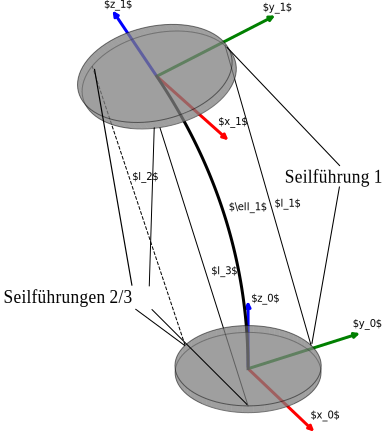
\includegraphics[width=.48\linewidth]{bilder/standdertechnik/continuum_robot3d.pdf}}
\begin{figure}[htb!]
\begin{subfigure}[t]{0.48\textwidth}
% füge bild ein, indem im Verhältnis zur definierten Box das Bild verschoben wird
\centering\raisebox{\dimexpr.5\ht\imagebox-.5\height}{
	\def\svgwidth{\textwidth}
	\input{bilder/standdertechnik/base.pdf_tex}
}
\caption{Trennscheibe der Roboterbasis}
\end{subfigure}
\begin{subfigure}[t]{0.48\textwidth}
\centering
\def\svgwidth{\textwidth}
\input{bilder/standdertechnik/continuum_robot3d.pdf_tex}
\caption{Segment des seilzugaktuierten kontinuierlichen Manipulators mit zwei Trennscheiben}
\end{subfigure}
\caption[Formgebung des Kontinuumsroboter durch Seilzüge]{Formgebung des Kontinuumsroboter durch Seilzüge}
\label{fig:roboterdesign}
\end{figure}

Die Krümmung des Kontinuumsroboters, bedingt durch die Seillängen und den Abstand der Seilführungen zum zentralen Rückgrat $d$, lautet
\begin{align}
\kappa = 2\frac{\sqrt{l_1^2+l_2^2+l_3^2-l_1l_2-l_2l_3-l_1l_3}}{d(l_1+l_2+l_3)}.
\label{eq:kappa}
\end{align}

Der Rotationswinkel des Kontinuumsroboters aus der $x$-$z$-Ebene wird durch
\begin{align}
\phi = \tan^{-1}\left(\frac{\sqrt{3}}{3} \frac{l_3+l_2-2l_1}{l_2-l_3} \right)
\label{eq:phi}
\end{align}

ermittelt. Für die numerische Berechnung des Rotationswinkels wird die Erweiterung der inversen Tangensfunktion $atan2(x, y)$, die die Vorzeichen der beiden Funktionsargumente $x$ und $y$ berücksichtigt, verwendet. Dadurch lässt sich der Rotationswinkel auf den Wertebereich von $[0~2\pi]$ abbilden. Zuletzt wird die Segmentlänge 
\begin{align}
\ell = \dfrac{nd(l_1+l_2+l_3)}{\sqrt{l_1^2+l_2^2+l_3^2-l_1l_2-l_2l_3-l_1l_3}} 
\sin^{-1}\left( \frac{\sqrt{l_1^2+l_2^2+l_3^2-l_1l_2-l_2l_3-l_1l_3}}{3nd} \right)
\label{eq:ell}
\end{align}

bestimmt. Die Anzahl der Trennscheiben beträgt $n$. Mit~\eqref{eq:kappa},~\eqref{eq:phi},~\eqref{eq:ell} wird an dieser Stelle die vektorwertige Funktion
\begin{align}
\bm{f}_{\mathrm{s}} =
\begin{bmatrix}
\kappa \\ \phi \\ \ell
\end{bmatrix} = 
\begin{bmatrix}
2\frac{\sqrt{l_1^2+l_2^2+l_3^2-l_1l_2-l_2l_3-l_1l_3}}{d(l_1+l_2+l_3)} \\
\tan^{-1}\left(\frac{\sqrt{3}}{3} \frac{l_3+l_2-2l_1}{l_2-l_3} \right) \\
\dfrac{nd(l_1+l_2+l_3)}{\sqrt{l_1^2+l_2^2+l_3^2-l_1l_2-l_2l_3-l_1l_3}} 
\sin^{-1}\left( \frac{\sqrt{l_1^2+l_2^2+l_3^2-l_1l_2-l_2l_3-l_1l_3}}{3nd} \right)
\end{bmatrix}
\label{eq:fspezifisch_vektor}
\end{align}

der Vollständigkeit halber angegeben. Zwischen zwei Trennscheiben wird angenommen, dass die Seilzüge keine Krümmung aufweisen. Erhöht man die Anzahl der Führungsscheiben theoretisch mit~$\lim n\to \infty$ entspricht dies einer Formgebung des Manipulators mit sich kontinuierlich krümmenden Aktoren~\cite{JW06}. Der Fall $l_1=l_2=l_3$ entspricht der singulären Stellung mit $\kappa = 0$, welcher für die Transformationsmatrix im vorigen Abschnitt bereits behandelt wurde. Für den Nennerterm des ersten Faktors von~\eqref{eq:ell} folgt dementsprechend: $\sqrt{l_1^2+l_2^2+l_3^2-l_1l_2-l_2l_3-l_1l_3} = 0$. Damit wäre die Berechnung der Segmentlänge im singulären Fall anhand~\eqref{eq:ell} nicht möglich. Die Segmentlänge entspricht hier der Länge der einzelnen Seilzüge \mbox{$\ell= (l_1+l_2+l_3)/3 = l_1=l_2=l_3$}.

Für die roboterspezifische Kinematik ist eine konstante Segmentlänge eine häufig gestellte Annahme. Dadurch lassen sich nur zwei Seillängen pro Segment unabhängig voneinander einstellen. Die dritte ist durch die Zwangsbedingung der konstanten Segmentlänge vorbestimmt. 
Im Rahmen dieser Arbeit weist die Kinematik eine variable Segmentlänge auf. Dadurch ist jedes einzelne Segment ein- und ausfahrbar. Die roboterspezifische Kinematik richtet sich damit maßgeblich nach~\cite{JW06a}. Die Autoren modellieren die Kinematik eines aus mehreren Segmenten bestehenden, seilzugaktuierten Kontinuumsroboters. Insbesondere werden Aktorgrenzen für die Gelenkwinkel berücksichtigt, die nicht durch eine konstante Segmentlänge eingeschränkt sind. Die einstellbaren \mbox{Gelenkwinkel $l_1, l_2, l_3$} werden durch eine untere und obere Grenze $l_{\mathrm{min}}$ bzw. $l_{\mathrm{max}}$ beschränkt. 

Seilzüge können prinzipiell nur Zugkräfte aufbauen und wären somit nicht in der Lage, den kontinuierlichen Manipulator über Aufbringen von Druckkräften zu strecken. Zwei Möglichkeiten, Druckkräfte zu entwickeln, werden an dieser Stelle erwähnt, aber im Weiteren für die Modellierung der Kinematik nicht weiter berücksichtigt. Eine Realisierung von Druckkräften ist prinzipiell mit einer am Rückgrat angebrachten Federvorrichtung möglich. Diese wird in Abhängigkeit von den eingestellten Gelenkwinkeln gestaucht oder gestreckt. Alternativ können die Seilzüge antagonistisch angeordnet werden, um Druckkräfte aufzubauen.  \newline

Mit den Ergebnissen der letzten beiden Abschnitte kann die gesamte, direkte kinematische Kette  
\begin{align}
\bm{x}_\mathrm{E} = \bm{f}_\mathrm{u} \left( \bm{f}_\mathrm{s} \left( [l_1, l_2, l_3]^\transpose \right) \right)
\label{eq:kinematische_kette}
\end{align}

eines seilzugaktuierten Kontinuumsroboters für ein Segment gebildet werden. Die Kinematik für mehrere verknüpfte Segmente eines Kontinuumsroboters ist Gegenstand des nächsten Abschnitts.

\subsection{Vorwärtskinematik mehrerer Segmente eines Kontinuumsroboters}
\label{subsec:multikinematik}

In den letzten beiden Abschnitten wurde der Grundstein für die direkte Kinematik eines seilzugaktuierten Kontinuumsroboter gelegt. Die Ergebnisse werden genutzt, um die Vorwärtskinematik des kontinuierlichen Manipulators mit mehreren verbundenen Segmenten zu ermitteln. \newline

Mit einer Verkettung von insgesamt $j$ homogenen Transformationsmatrizen
\begin{align}
{}^{0}\bm{T}_j = {}^{0}\bm{T}_{1} {}^1\bm{T}_{2} \dots {}^{j-1}\bm{T}_{j}
\end{align}

lässt sich eine beliebige Lage entlang von $j$ Segmenten transformieren. In dieser Arbeit werden zwei verknüpfte Segmente modelliert, sodass für die Transformationsmatrix folgt: ${}^{0}\bm{T}_2 = {}^{0}\bm{T}_{1} {}^1\bm{T}_{2}$. Sechs Gelenkwinkel 
$\bm{q} = \left[l_{1,1}, l_{1,2}, l_{1,3}, l_{2,1}, l_{2,2}, l_{2,3} \right]^\transpose$
beschreiben die Lage des Endeffektors eindeutig. 
Der erste Index der Seillängen bestimmt das Segment, an dem der Seilzug endet. Der Segmentindex steigt auf, beginnend bei der Roboterbasis. Der zweite Index legt den Seilzug gemäß Bild~\mbox{\ref{fig:roboterdesign}\,(b)} fest. Aus den gegebenen Seillängen des ersten Segments lässt sich die roboterspezifische Kinematik direkt berechnen. Die effektiven Seillängen des zweiten Segments, die für die Berechnung der Bogenparameter nötig sind, lauten
\begin{align}
l_{2,i,\mathrm{e}} = l_{2,i} - l_{1,i}\text{\,},~ i = 1,2,3.
\label{eq:effektive_laenge}
\end{align}

Die Seilzüge beider Segmente verlaufen jeweils durch dieselben Seilführungen der Trennscheiben. Es wird angenommen, dass die Seilzüge der jeweiligen Segmente die Formgebung des anderen Segments nicht beeinflussen. Dies stellt eine starke Vereinfachung dar, welche im Allgemeinen nicht gültig ist~\cite{WIJ10}. Diese Vereinfachung wird jedoch in Kauf genommen, da das Erlernen der inversen Kinematik mit Mitteln des RL im Vordergrund steht und nicht eine möglichst realistische Gestaltung der Kinematik beabsichtigt wird. \newline

Damit ist die Vorwärtskinematik für einen seilzugaktuierten Kontinuumsroboter mit zwei Segmenten vollständig beschrieben. Die Inverskinematik wird im nächsten Unterabschnitt behandelt.





\subsection{Inverskinematik}
\label{subesc:inverse_kinematik}

Für serielle Roboter wie auch Kontinuumsroboter gestaltet sich die Ermittlung der inversen Kinematik im Allgemeinen komplizierter als die der direkten. Zwei bestehende Konzepte zur Berechnung der inversen Kinematik eines kontinuierlichen Manipulators werden in diesem Abschnitt vorgestellt. Als erstes wird eine geometrische Ermittlung erläutert. Im Anschluss wird die differentielle Inverskinematik über die Berechnung von Jacobi-Matrizen vorgestellt. \newline

Ordnet man einer gegebenen Endeffektorlage eine Gelenkwinkelkonfiguration zu, spricht man von der Invers- bzw. inversen Kinematik
\begin{align}
\bm{q}  = \bm{f}^{-1} \left( \bm{x}_{\mathrm{E}} \right), 
\label{eq:inverskinematik}
\end{align} 

wobei $\bm{f}^{-1}$ die inverse Funktion zu $\bm{f}$ darstellt. In Hinblick auf Kontinuumsroboter mit stückweise konstanter Krümmung lässt sich die Inverskinematik in einen roboterunabhängigen Teil
\begin{align}
\left[ \kappa, \phi, \ell \right]^\transpose = \bm{f}^{-1}_{\mathrm{u}} \left( \bm{x}_{\mathrm{E}} \right)
\end{align}

und einen roboterspezifischen Teil
\begin{align}
\bm{q} = \bm{f}^{-1}_{\mathrm{s}} \left( \kappa, \phi, \ell \right)
\end{align}

aufteilen. Damit sind alle kinematischen Komponenten von Bild~\ref{fig:kinematikraeume} definiert. \newline

Zunächst wird die geometrische Lösung der inversen Kinematik erläutert.
Die inverse, roboterspezifische Funktion eines seilzugaktuierten Manipulators ist in~\cite{JW06} gegeben. Die Seillängen für ein Segment lassen sich geometrisch in Abhängigkeit der Kreisbogenparameter wie folgt berechnen:
\begin{align}
\bm{f}^{-1}_{\mathrm{s}} \left( \kappa, \phi, \ell \right) = 
\begin{bmatrix}
l_1 \\ l_2 \\l_3 
\end{bmatrix} =
\begin{bmatrix}
2n \sin \left( \dfrac{\kappa c}{2n} \right) \left( \dfrac{1}{\kappa} - d \sin\phi \right) \\
2n \sin \left( \dfrac{\kappa c}{2n} \right) \left( \dfrac{1}{\kappa} + d \sin \left(\dfrac{\pi}{3} + \phi  \right) \right) \\
2n \sin \left( \dfrac{\kappa c}{2n} \right) \left( \dfrac{1}{\kappa} - d \cos \left(\dfrac{\pi}{6} + \phi  \right) \right) \\
\end{bmatrix}.
\label{eq:fInversSpezifisch}
\end{align}

Damit ist prinzipiell nur noch die Bestimmung der inversen, roboterunabhängigen Kinematik notwendig. Es sind resultierende Kreisbogenparameter aus einer gegebenen Endeffektorlage gesucht. Neppalli et al. beschreiben in~\cite{NCJW09} ein Verfahren zur geometrischen Ermittlung von Kreisbogenparametern $\kappa, \phi, \ell$ aus einer gegebenen Endeffektorposition für einen Kontinuumsroboter mit $j$ Segmenten. Die Autoren lösen das beschriebene Problem mittels mehrerer Algorithmen, die in Tabelle~\ref{tab:geometrischeInverseUnabhaengigeKinematik} mit ihren Ein- und Ausgangsgrößen zusammengefasst sind. Die gewonnenen Bogenparameter können mit~\eqref{eq:fInversSpezifisch} in Seillängen des Kontinuumsroboters umgerechnet werden. 

Ein Nachteil der vorgestellten geometrischen Bestimmung von Bogenparametern besteht darin, dass die Abstände zwischen den Endpositionen der Robotersegmente vorgegeben werden müssen, siehe Tabelle~\ref{tab:geometrischeInverseUnabhaengigeKinematik}\,(a). Des Weiteren berücksichtigt dieser Ansatz keine Aktorgrenzen. Zuletzt ist die Orientierung des Endeffektors nicht Teil der Kinematik. 
\begin{table}[htb!]
\caption[Generelles Vorgehen der geometrischen Bestimmung von Kreisbogenparametern]
{Generelles Vorgehen der geometrischen Bestimmung von Kreisbogenparametern anhand einer gegeben Endeffektorlage nach~\cite{NCJW09}}
\begin{tabular}{ l  p{7.5cm} | p{6.50cm}}
\label{tab:geometrischeInverseUnabhaengigeKinematik}	
& \multicolumn{1}{c}{Eingangsgrößen} & \multicolumn{1}{c}{Ausgangsgrößen}\\ \hline\hline
(a) & Endeffektorposition $\bm{x}_{\mathrm{E,p}} = \bm{x}_{j,\mathrm{p}}$, Abstände zwischen den Endpositionen der einzelnen Robotersegmente \mbox{$d_i = ||\bm{x}_{i,\mathrm{p}}-\bm{x}_{i\shortminus1,\mathrm{p}}||_2$,} \mbox{$i = 1, \dots j $}, mit $\bm{x}_{0,\mathrm{p}} = \bm{0}$ & Endpositionen $\bm{x}_{i,\mathrm{p}}$, $i = 1,\dots j \shortminus 1$ \\ \hline
(b) & Endpositionen $\bm{x}_{i,\mathrm{p}}$, $i = 1, \dots j$, welche in die Roboterbasis transformiert werden &  Bogenparameter $\kappa_i, \phi_i, \ell_i$, $i \shortequal 1,  \dots j$ unter Anwendung von (c)  \\ \hline
(c) & Beliebige Position $\bm{x}_{\mathrm{p}}$ &  Bogenparameter $\kappa, \phi, \ell$ in Bezug zur Roboterbasis \\ 
\end{tabular}
\end{table}

Der nächste Ansatz löst die differentielle Kinematik
\begin{align}
\dot{\bm{x}}_{\mathrm{E}} = \bm{J} \mkern-1mu( \bm{q} ) \bm{q}
\label{eq:differentielle_kinematik}
\end{align}

mit der Jacobi-Matrix $\bm{J}\mkern-1mu (\bm{q})$. Über eine Invertierung der Jacobi-Matrix lässt sich die inverse, differentielle Kinematik 
\begin{align}
\dot{\bm{q}} = \bm{J}^{-1} \mkern-1mu( \bm{q} ) \dot{\bm{q}}
\label{eq:differentielleinverse_kinematik}
\end{align}

ermitteln. Nach~\cite{JW06} wird die folgende kinematischen Kette
\begin{align}
\bm{x}_{\mathrm{E}} 
\stackrel{\bm{f}_{\mathrm{DH}}}{\parbox{1cm}{\leftarrowfill}} \bm{\theta}, \bm{d}
\stackrel{\bm{f}_1}{\parbox{1cm}{\leftarrowfill}} \kappa, \phi, c
\stackrel{\bm{f}_2}{\parbox{1cm}{\leftarrowfill}} \bm{l}
\label{eq:informationsfluss_jones_walker}
\end{align}

aufgestellt. Die vektorwertige Funktion $\bm{f}_2$ entspricht dabei der bereits aufgeführten roboterspezifischen Kinematik gemäß~\eqref{eq:fspezifisch_vektor}, welche die Seillängen~$\bm{l}$ in Bogenparameter übersetzt. Die ermittelten Bogenparameter werden zunächst in klassische \textit{Denavit-Hartenberg}-Parameter~$\bm{\theta, \bm{d}}$ mittels $\bm{f}_1$ transformiert. Diese können wiederum mit~$\bm{f}_{\mathrm{DH}}$ zur \textit{Bishop}-Transformationsmatrix, gegeben durch~\eqref{eq:T_bishop}, überführt werden. Dieses Vorgehen unterscheidet sich von der Bestimmung der direkten, roboterunabhängigen Kinematik in Abschnitt~\ref{subsec:unabhaengige_vorwaertskinematik}, bei der die Transformationsmatrix direkt aus Bogenparametern ermittelt wird. Aus den einzelnen kinematischen Komponenten ermitteln die Autoren über eine Verkettung der Jacobi-Matrizen
\begin{align}
\dot{\bm{x}}_{\bm{\mathrm{E}}} = \bm{J}_{\mathrm{DH}} \bm{J}_{\bm{f}_1} \bm{J}_{\bm{f}_2}  \dot{\bm{l}} 
= \bm{J}\mkern-1mu (\bm{l}) \dot{\bm{l}}
\label{eq:modulare_differentielle_kinematik}
\end{align}

die differentielle Kinematik. Der modulare Aufbau der differentiellen Kinematik erlaubt es, diverse Hardware-Designs, die lediglich eine Anpassung der spezifischen Funktion $\bm{f}_2$ benötigen, zu realisieren. Außerdem ist eine echtzeitfähige Steuerung der Kinematik mit
\begin{align}
\dot{\bm{l}} = \bm{J}^{+} \mkern-2mu(\bm{l}) \dot{\bm{x}}
\label{eq:inverse_differentielle_kinematik}
\end{align}

möglich. $\bm{J}^{+}$, die Pseudoinverse zu $\bm{J}$, ist eine Verallgemeinerung der inversen Matrix auf singuläre und nichtquadratische Matrizen. \newline

Es wurden zwei Wege aufgezeigt, mit denen die inverse Kinematik eines seilzugaktuierten, kontinuierlichen Manipulators umgesetzt werden kann. Als nächstes wird das \textit{Reinforcement Learning} (RL) vorgestellt, bevor die in diesem Werk erarbeitete Methode der Inverskinematik von existierenden Ansätzen abgegrenzt wird.






\section{Reinforcement Learning}
\label{sec:rl_allgemein}

Wesentliche Konzepte, Komponenten und Begriffe des RL werden in diesem Abschnitt erläutert. RL umfasst eine Sammlung von Methoden des maschinellen Lernens und der künstlichen Intelligenz. Die Grundidee des RL besteht darin, Software- oder Roboteragenten zu gestalten, die durch Interaktionen mit einer unbekannten Umgebung über Versuch und Irrtum eigenständiges Handeln erlernen und definierte Ziele erreichen. \textit{Markow-Entscheidungsprozesse} (MEP) bilden die Grundlage für die Interaktion des Agenten mit einer unbekannten Umgebung und für die mathematische Analyse von RL-Algorithmen. Die Wertfunktion ermöglicht eine Bewertung von Zuständen, anhand welcher optimales Handeln abgeleitet werden kann. Die Strategie des Agenten, welche direkt ermittelt werden kann, ordnet Zuständen Aktionen zu. Der Agent versucht, seine Belohnungen in Form eines zukünftigen, diskontierten Ertrags zu maximieren. Die Standardmethoden des RL stoßen bei hochdimensionalen, kontinuierlichen Problemen an ihre Grenzen. Künstliche Neuronale Netze (KNN) verschaffen Abhilfe durch ihre Fähigkeit, hochdimensionale Zusammenhänge mit verhältnismäßig wenigen Parametern approximieren zu können. Werden neuronale Netze im Kontext des RL verwendet, spricht man von \textit{deep Reinforcement Learning} (dRL). Der grundlegende Aufbau sowie die Funktionsweise von neuronalen Netzen wird beschrieben. Drei Beispiele von erfolgreichen RL-Anwendungen sind in Bild~\ref{fig:rl_beispiele} illustriert. Bei der ersten Nennung von übersetzten Fachbegriffen ist nachstehend das englische Original angegeben. 

% ordne dem größten Bild eine Box zu
\newsavebox{\imgbox}
\savebox{\imgbox}{\includegraphics[width=0.32\textwidth]{bilder/standdertechnik/space_invaders.png}}
\begin{figure}[htb!]
\centering
\begin{subfigure}[t]{0.32\textwidth}
	\centering
	\includegraphics[width=\textwidth]{bilder/standdertechnik/space_invaders.png}
	\caption{\textit{Space Invaders}~\cite{MKS+15}}
\end{subfigure}
\begin{subfigure}[t]{0.32\textwidth}
	% erhöhe die Position der kleineren Bilder in Abhängigkeit von der Box
	\centering\raisebox{\dimexpr.5\ht\imgbox-.5\height}{
	\includegraphics[width=\textwidth]{bilder/standdertechnik/alphazero_go.png}
	}
	\caption{\textit{AlphaGo Zero}~\cite{SSS+17}}
\end{subfigure}
\begin{subfigure}[t]{0.32\textwidth}
	% erhöhe die Position der kleineren Bilder in Abhängigkeit von der Box
	\centering\raisebox{\dimexpr.5\ht\imgbox-.5\height}{
	\includegraphics[width=\textwidth]{bilder/standdertechnik/ball_in_cup.png}
	}
	\caption{Ball in Becher~\cite{NU11}}
\end{subfigure}
\caption[Anwendungen des Reinforcement Learning]{RL-Anwendungen. (a) Mithilfe des \textit{Deep Q-network} ist es möglich, Computerspiele direkt über die Auswertung von Pixeln zu lernen. Zu sehen ist das Spiel \textit{Space Invaders}. (b) \textit{AlphaGo Zero} ist eine künstliche Intelligenz, die ohne menschliches Expertenwissen das chinesische Brettspiel \textit{Go} gemeistert hat, indem sie unzählige Male gegen eine Kopie von sich selbst spielt. \textit{AlphaGo Zeros} Elo-Zahl liegt weit über den von den besten menschlichen Spielern.\footnotemark (c) Ein serieller Roboter lernt ein Geschicklichkeitsspiel, bei dem ein über eine Schnur verbundener Ball durch geschicktes Werfen in den Becher fallen soll.}
\label{fig:rl_beispiele}
\end{figure}




\pagebreak
\subsection{Markow-Entscheidungsprozesse und die Agent-Umgebung-Interaktion}
\label{subsec:MEP}



Wie eingangs erwähnt können RL-Probleme als MEP beschrieben werden. Alle Komponenten des MEP werden in dem Tupel 
$(\mathcal{S}, \mathcal{A}, \mathcal{T}, \mathcal{R}, \gamma)$
zusammengefasst. Nach~\cite{ADBB17} lauten die einzelnen Elemente:
%%%%%%%%%%%%%%%%%%%%%%%%%%%%%%%%%%%%%%%%%%%%%%%%%%%%%%%%%%%%%%%%%
\footnotetext{https://www.goratings.org/en/ (aufgerufen am 20.08.2018)}
%%%%%%%%%%%%%%%%%%%%%%%%%%%%%%%%%%%%%%%%%%%%%%%%%%%%%%%%%%%%%%%%%
\begin{itemize}
\item eine endliche Menge von Zuständen $\mathcal{S}$ (\textit{states}), sowie eine Verteilung von Ausgangszuständen~$\rho(\bm{s}_0)$
\item eine endliche Menge von Aktionen $\mathcal{A}$ (\textit{actions})
\item die Transitionsdynamik $\mathcal{T}( \bm{s}_{t+1} | \bm{s}_t, \bm{a}_t)$, die dem Zustand-Aktion-Paar (\textit{state action pair}) zur Zeit $t$ einen resultierenden Zustand zum Zeitpunkt $t+1$ zuordnet. Die Transitionsdynamik ist dem Agenten im Allgemeinen nicht bekannt
\item eine sofortige, skalare Belohnung, gegeben durch die Funktion $\mathcal{R}(\bm{s}_t, \bm{a}_t, \bm{s}_{t+1})$. Die Belohnung ist hervorgerufen durch die Aktion $\bm{a}_t$ im Zustand $\bm{s}_t$ und der folgenden Transition zum Zustand $\bm{s}_{t+1}$
\item der Diskontierungsfaktor (\textit{discount factor}) $\gamma \in [0~1]$, der zukünftige Belohnungen gewichtet
\end{itemize}



MEP werden in episodische und fortlaufende Prozesse unterteilt. Episodische MEP enden in einem finalen Zustand mit der Episodendauer $T$, wohingegen fortlaufende Prozesse die Episodendauer $T = \infty$ besitzen. In dieser Arbeit werden episodische MEP betrachtet. Zu jedem, diskreten Zeitpunkt $t = 0,1,2,3\dots,T$ beobachtet der Agent einen durch die Umgebung gegebenen Zustand $\bm{s}_t \in \mathcal{S}$. Ausgehend von diesem Zustand führt der Agent autonom und bedingt durch seine Strategie $\pi$ die Aktion $\bm{a}_t \in \mathcal{A}$ aus, welche die Umgebung beeinflusst. Die Strategie gibt formal die Wahrscheinlichkeitsverteilung für Aktionen in Abhängigkeit vom Zustand an: 
$\pi \, :\, \mathcal{S} \rightarrow p(\mathcal{A}=\bm{a}|\mathcal{S})$. 
Die Umgebung geht aufgrund der vom Agenten getätigten Aktion in den Zustand $\bm{s}_{t+1}$ über. Der neue Zustand sowie die instantane Belohnung $r_{t+1} \in \mathcal{R}$ werden an den Agenten kommuniziert. Im Rahmen von RL wird mit dem Belohnungssignal das Ziel oder ein für den Agenten beabsichtigtes Handeln definiert. Im Gegensatz zu Zuständen und Aktionen, die verallgemeinert als Vektorgrößen dargestellt sind, ist die Belohnung immer skalar.
In Bild~\ref{fig:agent_umgebung} ist der typische Signalflussplan der Agent-Umgebung-Interaktion veranschaulicht. RL ist verwandt mit dem Forschungsfeld der optimalen Regelung. Die Begriffe Agent, Umgebung, Aktion werden im RL anstatt der analogen Ausdrücke Regler, Regelstrecke und Stellgröße verwendet~\cite{SB98}.
\begin{figure}[!b]
\centering
\def\svgwidth{0.8\textwidth}
\input{bilder/standdertechnik/agent_umgebung.pdf_tex}
\caption[Agent-Umgebung-Interaktion]{Agent-Umgebung-Interaktion am Beispiel des Navigierens durch ein Labyrinth. Das Ziel ist, das Labyrinth durch den gegenüberliegenden Ausgang zu verlassen. Der Zustand $\bm{s}_t$ könnte die aktuelle Position des Agenten beschreiben. Planare Bewegungen \textit{oben}, \textit{unten}, \textit{links} und \textit{rechts} bilden ein simples Beispiel für mögliche Aktionen $\bm{a}_t$ im Labyrinth. Die Strategie $\pi$ bestimmt die Aktion des Agenten. Im Fall der vorliegenden Navigationsaufgabe ist das konstante Belohnungssignal $r_t= \shortminus 1$ ein beliebter Anreiz, den Agenten zum Verlassen des Labyrinths zu bewegen. Denn je länger der Agent sich im Labyrinth befindet, desto mehr negative Belohnungen erhält er. Diese können als Bestrafungen aufgefasst werden.}
\label{fig:agent_umgebung}
\end{figure}
Die Abfolge eines MEP lautet
\begin{align*}
\bm{s}_0, \bm{a}_0, r_1, \bm{s}_1, \bm{a}_1, r_1, \bm{s}_2, \bm{a}_2, r_3, \dots, T
\end{align*}

und wird Trajektorie genannt. Während jeder Trajektorie akkumuliert der Agent den diskontierten Ertrag (\textit{return})
\begin{align}
G = \sum_{t=0}^{T-1} \gamma^t r_{t+1},
\label{eq:ertrag}
\end{align}

den er zu maximieren versucht. Im Hinblick auf die Strategie lautet das Ziel von RL, eine optimale Strategie $\pi_*$ zu finden, die den maximalen erwarteten Ertrag erzielt $\pi_* = \argmax_\pi \mathds{E}[G|\pi]$.
In~\eqref{eq:ertrag} sind zwei Grenzfälle in Abhängigkeit des Diskontierungsfaktor zu erkennen. Für $\gamma=0$ fließt nur die instantane Belohnung in den Ertrag ein. Im Gegensatz dazu werden für $\gamma = 1$ alle Belohnungen unabhängig vom Zeitpunkt ihres Eintreffens gleich bewertet. Der Diskontierungsfaktor verringert im Allgemeinen zukünftige Belohnungen. In fortlaufenden MEP ist $\gamma < 1$ notwendig, damit die Summe~\eqref{eq:ertrag} einen endlichen Wert aufweist. 
MEP liegt die \textit{Markow-Eigenschaft} zugrunde, die besagt, dass zum Erreichen eines Ziels nur das Wissen über den aktuellen Zustand notwendig ist~\cite{SB98}. Zustände, die in der Vergangenheit liegen, beeinflussen damit die Entscheidungsfindung des Agenten nicht. Die Navigationsaufgabe des Agenten in Bild~\ref{fig:agent_umgebung} dient als Beispiel für die \textit{Markow-Eigenschaft} von RL-Problemen. Um an das Ende eines Labyrinths zu gelangen, spielt es für den Agenten keine Rolle, wo er sich in der Vergangenheit aufgehalten hat. \newline

In diesem Abschnitt wurden die elementaren Rahmenbedingungen vom RL erläutert. In dieser Arbeit werden zwei Klassen von Methoden zur Lösung von RL-Problemen behandelt. Die erste befasst sich mit der Ermittlung von Wertfunktionen. Die zweite errechnet parametrierte Strategien. Beide Klassen werden nachstehend beschrieben.






\subsection{Wertfunktionen}
\label{subsec:wertfunktionen}

Ein wesentlicher Bestandteil von RL ist die Wertfunktion (\textit{value function}), die Zustände bzw. Zustand-Aktion-Paare (\textit{state action pairs}) durch die Zuordnung eines Skalars bewertet. Nahezu alle RL-Algorithmen beinhalten die Schätzung einer Wertfunktion~\cite{SB98}. Aus diesem Grund werden die wesentlichen Aspekte von Wertfunktionen zusammengefasst. \newline

Die Zustand-Wertfunktion (\textit{state-value function})
\begin{align}
V_\pi(\bm{s}) = \mathds{E}[G|\bm{s},\pi]
\label{eq:zustand_wertfunktion}
\end{align}

entspricht dem erwarteten Ertrag~\eqref{eq:ertrag}, wenn sich der Agent im Zustand $\bm{s}$ befindet und der Strategie $\pi$ folgt. Die Zustand-Wertfunktion ist ein allgemeines Maß dafür, welcher diskontierte, zukünftige Ertrag in bestimmten Zuständen zu erwarten ist. 
Die Zustand-Aktion-Wertfunktion, auch Q-Funktion genannt, (\textit{state-action-value function}) 
\begin{align}
Q_\pi (\bm{s}, \bm{a}) = \mathds{E}[G|\bm{s},\bm{a},\pi]
\label{eq:zustand_aktion_wertfunktion}
\end{align}

ähnelt~\eqref{eq:zustand_wertfunktion}. Der einzige Unterschied besteht darin, dass in~\eqref{eq:zustand_aktion_wertfunktion} eine auszuführende Aktion $\bm{a}$ im Zustand $\bm{s}$ gegeben ist. Nach Ausführung der Aktion wird die Strategie $\pi$ verfolgt.
Die optimale Strategie $\pi_*$ maximiert den erwarteten, zukünftigen Ertrag
\begin{align}
V_*	(\bm{s}) = \max\limits_{\pi} V_\pi (\bm{s}) \quad \forall \, \bm{s} \in \mathcal{S}.
\label{eq:v_optimal}
\end{align}

Ist $V_*(\bm{s})$ bekannt, wählt der Agent im Zustand $\bm{s}$ die Aktion $\bm{a}$, die $\mathds{E}[V_*(\bm{s}_{t+1})]$ maximiert.  Die optimale Strategie bezüglich der Zustand-Aktion-Wertfunktion wählt die Aktion $\bm{a}$ gierig (\textit{greedy}) im Hinblick auf alle vorhandenen Aktionen im Zustand $\bm{s}$:
$\argmax_{\bm{a}} Q_\pi (\bm{s}, \bm{a})$. Die $\argmax$-Funktion ermittelt die Aktion $\bm{a}$, die den ihr folgenden, mathematischen Ausdruck maximiert. Eine weitere wichtige Größe in RL-Algorithmen ist der Vorteil (\textit{advantage})
\begin{align}
A_\pi (\bm{s},\bm{a}) = Q_\pi(\bm{s}, \bm{a}) - V_\pi (\bm{s}). 
\label{eq:vorteil}
\end{align}

Im Gegensatz zu~\eqref{eq:zustand_wertfunktion} und~\eqref{eq:zustand_aktion_wertfunktion} gibt der Vorteil nicht einen absoluten, sondern einen relativen Wert an. Der Vorteil gibt darüber Auskunft, inwiefern die vom Agenten gewählten Aktion $\bm{a}$ ihn im Zustand $\bm{s}$ besser oder schlechter stellt. 

Die Methoden des dynamischen Programmierens ermöglichen im tabellarischen Fall, RL-Probleme rekursiv zu lösen. Hierbei wird die Markow-Eigenschaft genutzt, um die Zustand-Wertfunktion in Form einer Bellman-Gleichung
\begin{align}
V_\pi (\bm{s}_t) = \max\limits_{\bm{a}} \mathds{E}[r_{t+1} + \gamma V_\pi(\bm{s}_{t+1})]
\label{eq:bellman_v}
\end{align}

zu definieren. Ausgehend vom Zustand~$\bm{s}_t$ wird diejenige Aktion gewählt, die den Erwartungswert der sofortigen Belohnung sowie den diskontierten Wert des folgenden Zustands~$\bm{s}_{t+1}$ maximiert. Die Bellman-Gleichung für die Zustand-Aktion-Wertfunktion lautet:
\begin{align}
Q_\pi (\bm{s}_t, \bm{a}_t) = \mathds{E} \left[r_{t+1} + \gamma \max\limits_{\bm{a}_{t+1}} Q_\pi (\bm{s}_{t+1}, \pi(\bm{s}_{t+1})) \right].
\label{eq:bellman_q}
\end{align}

Die Gleichungen~\eqref{eq:bellman_v} und~\eqref{eq:bellman_q} werden mit der Methode des \textit{Bootstrapping} ermittelt. Das heißt, es wird eine aktuelle Schätzung der Wertfunktionen verwendet, um eine Verbesserung der jeweiligen Schätzungen zu bewerkstelligen. 

Die generalisierte Strategieiteration (\textit{generalized policy iteration}) beschreibt das Vorgehen zum Auffinden der optimalen Wertfunktion. Eine Iteration der Strategie besteht aus der Strategieevaluation (\textit{strategy evaluation}) und der Strategieverbesserung (\textit{strategy improvement}). Strategieevaluation schätzt die Wertfunktion für eine beliebige Strategie $\pi$. Eine Strategieverbesserung kann durch gieriges Handeln hinsichtlich der Wertfunktion erzielt werden. Das heißt der Agent wählt Aktionen, die den maximalen, erwarteten Ertrag zur Folge haben. 

Im tabellarischen Fall müsste man prinzipiell für jeden Zustand einen Eintrag im Speicher hinterlegen. Für Probleme mit wenigen Zuständen sind tabellarische Methoden in der Lage, optimale Lösungen zu finden. Sobald man jedoch versucht kontinuierliche Probleme zu lösen, ist die computergestützte, tabellarische Repräsentation von Zuständen nicht mehr realisierbar. 
%Das Spiel \textit{GO} weist beispielsweise $~2 * 10^170$ erlaubte Positionen auf. 
Aus diesem Grund werden Methoden der Funktionsapproximation herangezogen, die in Abschnitt~\ref{sec:knn} erläutert werden.\newline

Mithilfe von Wertfunktionen lassen sich Zustände bewerten und schließlich optimales Handeln des Agenten ableiten. Die zweite Methode, RL-Probleme zu lösen, folgt im nächsten Unterabschnitt.






\subsection{Strategiesuche}
\label{subsec:strategiesuche}

Bei der Strategiesuche wird direkt eine optimale Strategie gesucht, anstatt diese über die Ermittlung der Wertfunktion abzuleiten. Strategien werden üblicherweise mit einem Satz von Parametern $\bm{\theta}$ beschrieben. Eine parametrierte Strategie $\pi_{\bm{\theta}}$ wählt Aktionen hinsichtlich ihrer Parameter und wird mit dem entsprechenden Subskript versehen. Das Ziel der Strategiesuche besteht darin, den erwarteten Ertrag 
$\mathds{E}[G|\bm{\theta}]$ 
durch entsprechende Parameteraktualisierungen zu maximieren. Es existieren gradientenfreie und gradientenbasierte Verfahren zur Optimierung von parametrierten Strategien, wobei letztere im Vordergrund dieser Arbeit stehen. \newline

Strategien $\pi(\bm{a}|\bm{s},\bm{\theta})$ können prinzipiell beliebig parametriert werden, solange sie differenzierbar hinsichtlich ihrer Parameter sind. Folglich existiert der Gradient $\nabla_{\bm{\theta}}\pi(\bm{a}|\bm{s},\bm{\theta})$ und ist endlich, mit $\nabla_{\bm{\theta}}$, dem Nabla-Operator hinsichtlich der Parameter $\bm{\theta}$.  Die gradientenbasierte Parameteraktualisierung wird mittels des Gradientenaufstiegs (\textit{gradient ascent})
\begin{align}
\bm{\theta}_{t+1} = \bm{\theta}_t + \alpha \nabla_{\bm{\theta}} \bm{L}(\bm{\theta}_t)
\label{eq:parameterupdate}
\end{align}

bewerkstelligt. Die Kostenfunktion $\bm{L}(\bm{\theta})$ beinhaltet meist eine Form des erwarteten Ertrags sowie der parametrierten Strategie. Die Lernrate $\alpha$ skaliert die Parameteraktualisierung und nimmt üblicherweise einen Wert $\alpha \ll 1$ an. Strategiegrandientenmethoden (\textit{policy gradient methods}) werden alle Verfahren genannt, welche die Parameteraktualisierung~\eqref{eq:parameterupdate} verwenden. 
Die Ausgangsgrößen von stochastischen Strategien (\textit{stochastic policies}) berechnen die Parameter einer Wahrscheinlichkeitsverteilung, z.\,B. den Erwartungswert und die Standardabweichung der Gaußschen Normalverteilung. Damit ist die Strategie in der Lage, Werte für die Aktionen des Agenten direkt zu errechnen. 

Das gradientenbasierte Strategie-Theorem (\textit{policy gradient theorem}) liefert einen analytischen Ausdruck für den Gradienten der Kostenfunktion hinsichtlich ihrer Parameter~\cite{SB98}. Die Parameteraktualisierung des REINFORCE-Algorithmus~\cite{Wil92} 
\begin{align}
\bm{\theta}_{t+1} = \bm{\theta}_t + \alpha G_t 
\dfrac{\nabla_{\bm{\theta}} \pi(\bm{a}_t|\bm{s}_t, \bm{\theta}_t)}{\pi(\bm{a}_t|\bm{s}_t, \bm{\theta}_t)}
\label{eq:REINFORCE}
\end{align}

wird aufgrund ihrer veranschaulichenden Wirkung beispielhaft aufgeführt. Die Parameterveränderung ist proportional zu dem Produkt aus dem Ertrag $G_t$ und einem Vektor, dem Gradienten der Wahrscheinlichkeit, eine Aktion auszuführen, dividiert durch die Wahrscheinlichkeit, die Aktion zu wählen. Der Vektor zeigt in die Richtung des steilsten Anstiegs im Parameterraum, dieselbe Aktion im selben Zustand zu wiederholen. Das heißt, \eqref{eq:REINFORCE} verändert die Wahrscheinlichkeit von Aktionen proportional zum Ertrag. Aktionen, die einen geringen Ertrag liefern, werden nach der Parameteraktualisierung unwahrscheinlicher gemacht. Wiederum wird die Wahrscheinlichkeit von Aktionen, die einen hohen Ertrag erzielen, erhöht. Der Ausdruck im Nenner sorgt dafür, dass seltene Aktionen berücksichtigt werden. Ansonsten werden wahrscheinlich eintretende Aktionen mit möglicherweise geringem Ertrag bevorzugt. \newline

Wertfunktionen sowie Strategien kontinuierlicher und hochdimensionaler RL-Probleme werden parametriert und approximiert. Künstliche neuronale Netze stellen eine Möglichkeit dar, Funktionen zu approximieren.





\section{Künstliche neuronale Netzwerke}
\label{sec:knn}

Der Gebrauch von KNN in Verbindung mit RL ermöglicht das Lösen von komplizierten, hochdimensionalen Problemen~\cite{ADBB17}. Die Fähigkeit von KNN, komplexe Zusammenhänge mit relativ wenigen Parametern repräsentieren zu können, spielt hierbei eine bedeutende Rolle.  
%Besondere Erfolge wurden in der Bildverarbeitung, Spracherkennung und -übersetzung verbucht~\cite{GBC16}. 
%Im Folgenden werden die grundlegenden Elemente und Funktionsweisen eines KNN dargelegt. 
In diesem Abschnitt wird zunächst der generelle Aufbau von KNN erläutert. Anschließend werden einige wichtige Aktivierungs- bzw. Transformationsfunktionen vorgestellt. Der \textit{Backpropagation}-Algorithmus, nachfolgend \textit{Backpropagation} genannt, wird verwendet, um das Erlernen von Zusammenhängen durch KNN zu ermöglichen. 






\subsection{Netzwerkarchitektur und Vorwärtspass}
\label{subsec:architektur_vorwaertspass}

In Verbindung mit RL stechen zwei häufig applizierte Netzwerkarchitekturen hervor: neuronale Vorwärtsnetzwerke (\textit{feedforward neural nets}) und neuronale Faltungsnetzwerke (\textit{convolutional neural nets}). Die Architektur bestimmt die Funktionsweise des Netzwerks. Vorwärtsnetzwerke errechnen die formale Beziehung
$\bm{y} = f(\bm{x};\bm{\theta})$,
welche den funktionalen Zusammenhang zwischen dem Eingangssignal $\bm{x}$ und dem Ausgangssignal $\bm{y}$ approximiert. Die zu lernenden Parameter sind $\bm{\theta}$. Werden Vorwärtsnetzwerke zusätzlich mit Faltungsschichten (\textit{convolutional layers}) versehen, spricht man von Faltungsnetzwerken. In der Bild- und Sprachverarbeitung ist die Verwendung von Faltungsoperationen relevant, da dadurch niedrigdimensionale Merkmale (\textit{features}) aus hochdimensionalen Daten extrahiert werden können. Nachfolgend wird der Fokus auf Vorwärtsnetzwerke gelegt. 
\newline

Vorwärtsnetzwerke besitzen eine Eingangs- und Ausgangsschicht (\textit{input and output layer}) sowie mindestens eine versteckte Schicht (\textit{hidden layer}). Bild~\ref{fig:knn} illustriert ein flaches Vorwärtsnetzwerk mit einer versteckten Schicht. Jeder Kreis repräsentiert ein Neuron, die kleinste Einheit des KNN. Ein Netz heißt dicht oder dicht vernetzt, wenn alle Neuronen einer Schicht Verbindungen zu allen Neuronen der folgenden Schicht aufweisen. Tiefe Vorwärtsnetzwerke besitzen mindestens zwei versteckte Schichten. 
\begin{figure}[h]
\centering
\def\svgwidth{0.7\textwidth}
\input{bilder/standdertechnik/knn.pdf_tex}
\caption[Dicht vernetztes, flaches Vorwärtsnetzwerk]{Dicht vernetztes, flaches Vorwärtsnetzwerk}
\label{fig:knn}
\end{figure}

Während die Dimensionalität des Ein- und Ausgangssignals durch äußere Rahmenbedingungen vorgegeben ist, hängt die Dimension der Wichtungsmatrizen $\bm{W}$ und Voraktivierungen $\bm{b}$ von der gewählten Anzahl der Neuronen ab. Neuronen sind skalare Matrix- bzw. Vektoreinträge, die während des Trainings des Netzes angepasst werden, sodass sie definierte Kostenfunktionen maximieren oder minimieren. Das Eingangssignal wird durch das Netzwerk mittels Matrix-Vektormultiplikation und Aktivierungsfunktionen geleitet und transformiert, sodass schließlich das Ausgangssignal errechnet wird. Dieser Vorgang nennt sich Vorwärtspass (\textit{forward pass}) und ist in Algorithmus~\ref{alg:vorwaertspass} mit seinen mathematischen Operationen aufgeführt. 
\begin{algorithm}[!htb]
\caption[Vorwärtspass eines dicht vernetzten Vorwärtsnetzwerks]{Vorwärtspass eines dicht vernetzten Vorwärtsnetzwerks in Anlehnung an~\cite{GBC16}. Die zu lernenden Parameter $\bm{\theta}$ sind in den Wichtungsmatrizen $\bm{W}_i$ und den Voraktivierungen $\bm{b}_i$ (\textit{bias}) enthalten. Nach einer Multiplikation des vektorwertigen Signals $\bm{h}_{i-1}$ mit der Wichtungsmatrix $\bm{W}_i$ wird die Voraktivierung $\bm{b}_i$ addiert. Die resultierende Summe wird durch die nichtlineare Aktivierungsfunktion $g(\bm{z}_i)$ transformiert. Dieser Vorgang wird solange wiederholt, bis alle Schichten des Netzwerks passiert sind und das Ausgangssignal $\bm{y}$ ermittelt ist.}
\label{alg:vorwaertspass}
\begin{algorithmic}[1]
\Require Netzwerktiefe $k$
\Require Wichtungsmatrizen $\bm{W}_i, i \in \{1, \dots, k\}$
\Require Voraktivierungen $\bm{b}_i, i \in \{1, \dots, k\}$
\Require Aktivierungsfunktionen $g_i(\bm{z}), i \in \{1, \dots, k\}$
\Require Eingangssignal $\bm{x}$
\State $\bm{h}_0 = \bm{x}$
\For{i=1, \dots, k} 
%	\State $\bm{z}_i = \bm{b}_i + \bm{W}_i \bm{h}_{i-1}$
	\State $\bm{h}_i = g_i(\bm{W}_i \bm{h}_{i-1} + \bm{b}_i)$
\EndFor
\State $\bm{y} = \bm{h}_k$
\end{algorithmic}
\end{algorithm}







\subsection{Nichtlineare Aktivierungen}
\label{subsec:nichtlineare_aktivierung}

Ein entscheidender Vorgang des Vorwärtspasses bildet die nichtlineare Aktivierung, welche die Approximation von nichtlinearen Zusammenhängen erst ermöglicht, da der Vorwärtspass sonst nur aus einer Kombination von linearen Funktion bestehen würde. In diesem Unterabschnitt werden drei relevante Aktivierungsfunktionen vorgestellt. \newline

\textit{Rectified linear units} (ReLU) besitzen die Aktivierungsfunktion $g(z) = max\{0,z\}$ und werden von Goodfellow et al. als Standardaktivierungen für die versteckten Schichten von KNN vorgeschlagen. ReLU bilden eine stückweise lineare Funktion, wodurch sie viele Eigenschaften bewahren, die die Optimierung mittels gradientenbasierter Verfahren vereinfacht~\cite{GBC16}.

Die nichtlineare Aktivierung der Ausgangsschicht ist optional und hängt von dem zu approximierenden Sachverhalt ab. Für Klassifizierungsprobleme mit nur zwei Kategorien kann die logistische Sigmoidfunktion $g(z) = 1/(1+\exp(-z))$ eingesetzt werden.
Sigmoidfunktionen bilden eine Klasse von Funktionen mit S-förmigen Graphen. Die logistische Sigmoidfunktion besitzt den Wertebereich $g(z)\in[ 0~1]$, wodurch das Ergebnis als Wahrscheinlichkeit, eine von zwei Klassen identifiziert zu haben, interpretiert werden kann. 


Möchte man mit einem KNN bspw. ein Beschleunigungs- oder Bremssignal mithilfe eines Skalars approximieren, wobei positive Werte eine Beschleunigung und negative eine Bremsung hervorrufen, kann man den Tangens hyperbolicus als Aktivierungsfunktion verwenden. Dieser liefert Werte zwischen $\shortminus 1$ und $1$. 

Die drei vorgestellten Aktivierungsfunktionen sind in Bild~\ref{fig:aktivierungen} dargestellt. 
Das universale Approximationstheorem (\textit{universal approximation theorem}) besagt, dass ein Vorwärtsnetzwerk mit einer versteckten Schicht, einer nichtlinearen Aktivierung und einer finiten Anzahl von Neuronen beliebige, kontinuierliche Funktionen approximieren kann. 
Für Sigmoidfunktionen hat Cybenko in~\cite{Cyb89} und für ReLU haben Leshno et al. in~\cite{LLPS93} das Theorem nachgewiesen.

\begin{figure}[!htb]
\centering
\begin{subfigure}{.32\textwidth}
	\centering
	\begin{tikzpicture}
	\begin{axis}[xmax=3, xmin=-3, ymax=1, ymin=-1, samples=50, width=\textwidth]
		\addplot[imesblue, ultra thick][domain=-3:0] {0};
		\addplot[imesblue, ultra thick][domain=0:3] {x};
	\end{axis}	
	\end{tikzpicture}
	\caption{ReLU}
\end{subfigure}
\begin{subfigure}{.32\textwidth}
	\centering
	\begin{tikzpicture}
	\begin{axis}[xmax=3, xmin=-3, ymax=1, ymin=-1, samples=50, width=\textwidth]
		\addplot[imesblue, ultra thick] {1/(1+ exp(-x) )};
	\end{axis}	
	\end{tikzpicture}
	\caption{Logistische Sigmoidfunktion}
\end{subfigure}
\begin{subfigure}{.32\textwidth}
	\centering
	\begin{tikzpicture}
	\begin{axis}[xmax=3, xmin=-3, ymax=1, ymin=-1, samples=50, width=\textwidth]
		\addplot[imesblue, ultra thick] {tanh(x)};
	\end{axis}	
	\end{tikzpicture}
	\caption{Tangens hyperbolicus}
\end{subfigure}
\caption{Drei relevante Aktivierungsfunktionen}
\label{fig:aktivierungen}
\end{figure}





\subsection{Backpropagation}
\label{subsec:backprop}

Wie bereits erwähnt werden Wertfunktionen oder Strategien im RL mit KNN approximiert. 
Ein KNN, welches eine Strategie repräsentiert, errechnet im Vorwärtspass aus einem Zustand des Agenten die dazugehörige Aktion. Die ermittelte Aktion hat Auswirkungen auf den resultierenden Ertrag und folglich auch auf die Parameteraktualisierung und Kostenfunktion in~\eqref{eq:parameterupdate} bei der Strategiesuche. Das Ziel der Strategiesuche besteht darin, die Parameter $\bm{\theta}$ zu erlernen, die den zukünftigen, erwarteten Ertrag maximieren. Dafür wird der Gradient der Kostenfunktion hinsichtlich der zu lernenden Parameter benötigt. 
Backpropagation wird verwendet, um Informationen rückwärts durch das Netzwerk fließen zu lassen und die notwendigen Gradienten zu ermitteln. 
Formal ermittelt Backpropagation den Gradienten $\nabla_{\bm{\theta}} \bm{L}(\bm{\theta})$ unter Anwendung der Kettenregel der Differentiation. Auf eine detaillierte Beschreibung von Backpropagation wird an dieser Stelle verzichtet, da Software-Bibliotheken des maschinellen Lernens eigenständig den Gradienten der Kostenfunktion in Abhängigkeit vom Vorwärtsnetzwerk ermitteln können. Für die Lösung eines RL-Problems steht die Gestaltung des Vorwärtspasses dabei im Vordergrund. \newline
